
% poo
\begin{frame}
  \begin{columns}[c]

    
    \begin{column}{0.3\textwidth}
      \centering
      \includegraphics[width=1\textwidth]{cow.png}
    \end{column}

    \begin{column}{0.8\textwidth}
      \centering
      \resizebox{3cm}{!}{
      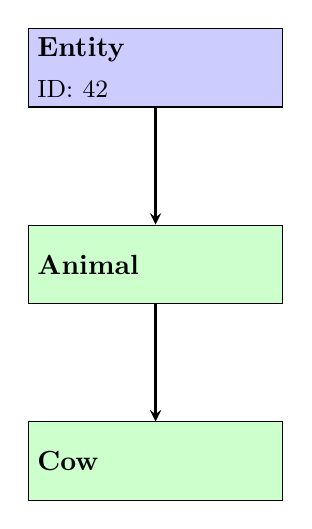
\begin{tikzpicture}[
        node distance=2.5cm,
        class/.style={rectangle, draw, fill=blue!10, text width=3cm, align=left, minimum height=1cm},
        arrow/.style={->, >=stealth, thick}
      ]
        % Entity
        \node[class, fill=blue!20] (entity) {\textbf{Entity}\\[0.1cm]\small ID: 42};
        
        % Components
        \node[class, fill=green!20, below of=entity] (animal) {\textbf{Animal}\\[0.1cm]\small};
        \node[class, fill=green!20, below of=animal] (cow) {\textbf{Cow}\\[0.1cm]\small};
                
        % Arrows
        \draw[arrow] (entity) -- (animal) node[midway, right, draw=none]{};
        \draw[arrow] (animal) -- (cow) node[midway, right, draw=none]{};
        
      \end{tikzpicture}
      }
    \end{column}
  \end{columns}
\end{frame}
% end poo

\begin{frame}
  \frametitle{Traditional OOP Approach}
  \framesubtitle{Inheritance Hierarchy}
  
  \begin{columns}[c]
    \begin{column}{0.2\textwidth}
      \centering
      \includegraphics[width=0.9\textwidth]{cow.png}
    \end{column}

    \begin{column}{0.7\textwidth}
      \centering
      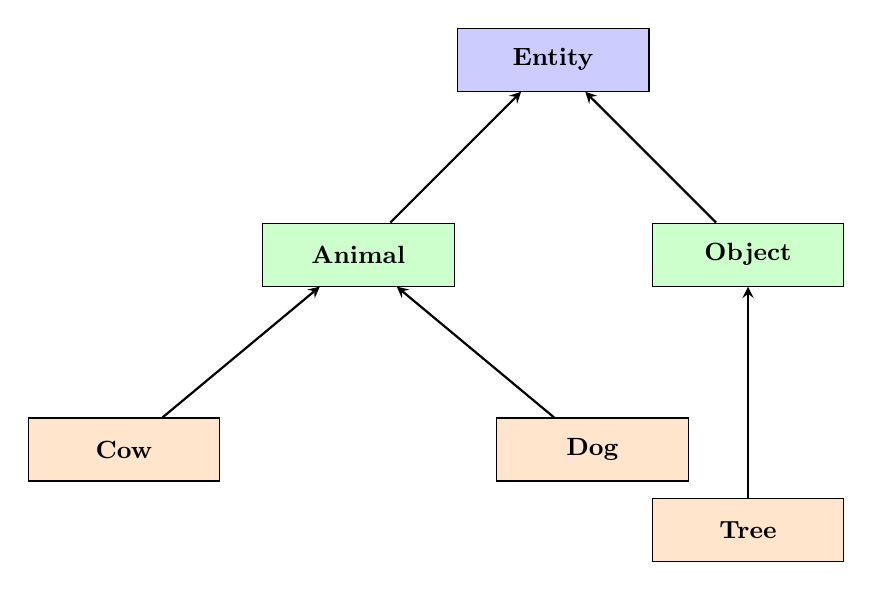
\begin{tikzpicture}[
        node distance=3.5cm and 2cm,
        class/.style={rectangle, draw, fill=blue!10, text width=2.2cm, align=center, minimum height=0.8cm, font=\small},
        arrow/.style={->, >=stealth, thick}
      ]
        % Top level
        \node[class, fill=blue!20] (entity) {\textbf{Entity}};
        
        % Second level
        \node[class, fill=green!20, below left of=entity] (animal) {\textbf{Animal}};
        \node[class, fill=green!20, below right of=entity] (object) {\textbf{Object}};
        
        % Third level - under Animal
        \node[class, fill=orange!20, below left of=animal, xshift=-0.5cm] (cow) {\textbf{Cow}};
        \node[class, fill=orange!20, below right of=animal, xshift=0.5cm] (dog) {\textbf{Dog}};
        
        % Third level - under Object
        \node[class, fill=orange!20, below of=object] (tree) {\textbf{Tree}};
        
        % Arrows
        \draw[arrow] (animal) -- (entity);
        \draw[arrow] (object) -- (entity);
        \draw[arrow] (cow) -- (animal);
        \draw[arrow] (dog) -- (animal);
        \draw[arrow] (tree) -- (object);
      \end{tikzpicture}
    \end{column}
  \end{columns}
  
  \vspace{0.3cm}
  \centering
  \small \textit{Traditional class inheritance creates rigid hierarchies}
\end{frame}
